\documentclass[11pt,leqno]{article}
\usepackage[spanish,activeacute]{babel}
\usepackage[utf8]{inputenc}
\usepackage{etex}
\usepackage{amsfonts}
\usepackage{enumerate}
\usepackage{listings}
\usepackage{amsthm}
\usepackage[hidelinks]{hyperref}
\usepackage{booktabs}
\usepackage{siunitx}
\usepackage{pgfplotstable}
\usepackage{verbatim}
\usepackage{geometry}
\usepackage{changepage}
\usepackage{pgfplots}
\usepackage{float}


\author{Jacinto Carrasco Castillo 	\\
		N.I.F. 32056356-Z			\\ 
		\href{jacintocc@correo.ugr.es}{jacintocc@correo.ugr.es}}
		
\title{	Práctica 1 Metaheurísticas.\\
		Búsqueda por trayectorias para el problema \\
		de la selección de características}

\newcommand{\maketable}[1]{
\begin{adjustwidth}{-1cm}{}
\resizebox{\linewidth}{!}{
\pgfplotstabletypeset[
	every head row/.style={
		before row={%
				\hline
				& \multicolumn{4}{c|}{WDBC} & \multicolumn{4}{c|}{Movement Libras} & \multicolumn{4}{c|}{Arrhythmia}\\
				\cline{2-13}
		},
		after row=\cline{2-13}\hline,
		column type=c
	},
	every first column/.style={ column type/.add={|}{} },
	every last row/.style={before row =\hline\hline, after row=\hline},
	column type/.add={}{|},
	columns/partition/.style={column name = , string type},
	columns/in/.style={column name =\%Clas. in},
	columns/inL/.style={column name =\%Clas. in},	
	columns/inA/.style={column name =\%Clas. in},
	columns/out/.style={column name =\%Clas. out},
	columns/outL/.style={column name =\%Clas. out},	
	columns/outA/.style={column name =\%Clas. out},
	columns/T/.style={column name =T},
	columns/tA/.style={column name =T},
	columns/tL/.style={column name =T},
	columns/red./.style={column name =\%red.},
	columns/redL/.style={column name =\%red.},	
	columns/redA/.style={column name =\%red.},
	precision=4
	]{#1}
}
\end{adjustwidth}
}

\newcommand{\makeresume}[4]{
\pgfplotstablevertcat{#1}{#2}
\pgfplotstablecreatecol[copy column from table={#3}{in}]{inL} {#1}
\pgfplotstablecreatecol[copy column from table={#3}{out}]{outL} {#1}
\pgfplotstablecreatecol[copy column from table={#3}{red}]{redL} {#1}
\pgfplotstablecreatecol[copy column from table={#3}{T}]{tL} {#1}
\pgfplotstablecreatecol[copy column from table={#4}{in}]{inA} {#1}
\pgfplotstablecreatecol[copy column from table={#4}{out}]{outA} {#1}
\pgfplotstablecreatecol[copy column from table={#4}{red}]{redA} {#1}
\pgfplotstablecreatecol[copy column from table={#4}{T}]{tA} {#1}
}

\newcommand{\getElement}[3]{\pgfplotstablegetelem{#2}{#3}\of{#1} \pgfplotsretval}


\begin{document}

% Tablas KNN
\pgfplotstableread[col sep=comma]{Resultados/wKNN.csv}\datawKNN
\pgfplotstableread[col sep=comma]{Resultados/lKNN.csv}\datalKNN
\pgfplotstableread[col sep=comma]{Resultados/aKNN.csv}\dataaKNN
   
% Tablas Greedy SFS
\pgfplotstableread[col sep=comma]{Resultados/wSFS.csv}\datawSFS
\pgfplotstableread[col sep=comma]{Resultados/lSFS.csv}\datalSFS
\pgfplotstableread[col sep=comma]{Resultados/aSFS.csv}\dataaSFS

% Tablas Local Search
\pgfplotstableread[col sep=comma]{Resultados/wLS.csv}\datawLS
\pgfplotstableread[col sep=comma]{Resultados/lLS.csv}\datalLS
\pgfplotstableread[col sep=comma]{Resultados/aLS.csv}\dataaLS

% Tablas Simulated Annealing
\pgfplotstableread[col sep=comma]{Resultados/wSA.csv}\datawSA
\pgfplotstableread[col sep=comma]{Resultados/lSA.csv}\datalSA
\pgfplotstableread[col sep=comma]{Resultados/aSA.csv}\dataaSA

% Tablas Tabu Search
\pgfplotstableread[col sep=comma]{Resultados/wTS.csv}\datawTS
\pgfplotstableread[col sep=comma]{Resultados/lTS.csv}\datalTS
\pgfplotstableread[col sep=comma]{Resultados/aTS.csv}\dataaTS

% Tablas Extended Tabu Search
\pgfplotstableread[col sep=comma]{Resultados/wETS.csv}\datawETS
\pgfplotstableread[col sep=comma]{Resultados/lETS.csv}\datalETS
\pgfplotstableread[col sep=comma]{Resultados/aETS.csv}\dataaETS


\maketitle

\begin{center}
Curso 2015-2016\\

Problema de Selección de Características.\\ 

Grupo de prácticas: Viernes 17:30-19:30\\

Quinto curso del Doble Grado en Ingeniería Informática y Matemáticas.\\
\textit{ }\\
\end{center}

Algoritmos considerados:
\begin{enumerate}
\item Greedy Sequential Forward Selection.
\item Búsqueda Local.
\item Enfriamiento Simulado.
\item Búsqueda Tabú Básica.
\item Búsqueda Tabú Extendida.
\end{enumerate}

\newpage

\tableofcontents
\newpage

\section{Descripción del problema}

El problema que nos ocupa es un problema de clasificación. Partimos de una muestra de los objetos que queremos clasificar y su clasificación, es decir, la clase a la que pertenece y pretendemos, en base a esta muestra, poder clasificar nuevas instancias que nos lleguen.\\
La clasificación se realizará en base a una serie de características, que nos permitan determinar si un individuo pertenece a un grupo u otro. Por tanto, tendremos individuos de una población $\Omega$ representados como un vector de características: $ \omega \in \Omega; \omega = (x_1(\omega), \dots x_n(\omega))$, donde $\omega$ es un individuo de la población y $x_i, i=1,\dots n$ son las $n$ características sobre las que se tiene información. Buscamos $f:\Omega \longrightarrow C=\{C_1, \dots, C_M\}$, donde $C=\{C_1, \dots, C_M\}$ es el conjunto de clases a las que podemos asignar los objetos.\\
El problema de clasificación está relacionado con la separabilidad de las clases en el sentido de que existirá la función $f$  anteriormente mencionada siempre que las clases sean separables, es decir, siempre que un individuo con unas mismas características pertenzcan a una misma clase. Sin embargo, si se da que dos individuos $\omega_1, \omega_2 \in \Omega$, $(x_1(\omega_1), \dots x_n(\omega_1))=(x_1(\omega_2), \dots x_n(\omega_2))$ y sin embargo $f(\omega_1) \neq f(\omega_2)$, no podrá existir $f$. En todo caso, querríamos obtener la mayor tasa de acierto posible.\\  
Por tanto, queremos, en base a unos datos, hallar la mejor $f$ posible. De esto trata el aprendizaje clasificado: Se conocen instancias de los datos y las clases a las que pertenecen. Usaremos como técnica de aprendizaje supervisado la técnica estadística conocida como $k$ vecinos más cercanos. Se trata de buscar los $k$ vecinos más cercanos y asignar al objeto la clase que predomine de entre los vecinos. En caso de empate, se seleccionará la clase con más votos más cercana.\\  
Pero no nos quedamos en el problema de clasificación, sino que buscamos reducir el número de características. Con esto pretendemos seleccionar las características que nos den un mejor resultado (por ser las más influyentes a la hora de decidir la categoría). Usaremos los datos de entrenamiento haciendo pruebas mediante diferentes metaheurísticas hasta obtener la mejor selección que seamos capaces de encontrar.\\  
El interés en realizar la selección de características reside en que se aumentará la eficiencia, al requerir menos tiempo para construir el clasificador, y que se mejoran los resultados al descartar las características menos influyentes y que sólo aportan ruido. Esto hace también que se reduzcan los costes de mantenimiento y se aumente la interpretabilidad de los datos.\\
Las funciones de evaluación pueden estar basadas en la consistencia, en la Teoría de la Información, en la distancia o en el rendimiento de clasificadores. Nosotros usaremos el rendimiento promedio de un clasificador $3-NN$.


\section{Descripción de la aplicación de los algoritmos}
\subsection{Representación de soluciones}
	Para este problema tenemos varias formas posibles de representar las soluciones:
	\begin{itemize}
		\item Representación binaria: Cada solución está representada por un vector binario de longitud igual al número de características, donde las posiciones seleccionadas tendrán un 1 o $\texttt{True}$ y las no seleccionadas un 0 o $\texttt{False}$. Esta opción, que será la que tomaremos, sólo es recomendable si no tenemos restricciones sobre el número de características seleccionadas.
		\item Representación entera: Cada solución es un vector de tamaño fijo $m \leq n$ con las características seleccionadas. Esta representación sí es adecuada si tenemos restricciones sobre el número de características tomadas ya que no podemos hacerlo con más de $m$.
		\item Representación de orden: Cada solución es una permutación de $n$ elementos, ordenados según la importancia de cada característica. Aquí también se maneja el cumplimiento de restricciones pues una vez encontrada la solución, tomaremos sólo las primeras $m$ características.
	\end{itemize}
	Se ha de mencionar que en las dos últimas representaciones el espacio de soluciones es mayor que el espacio de búsqueda, justificado en la representación de orden porque da más información (podríamos tomar soluciones de longitud variable), pero que en la representación entera sólo es razonable asumir si tenemos una restricción de longitud fija. Además, otra ventaja de la representación binaria es la facilidad para aplicarle operadores (de vecindario, en posteriores prácticas de cruce...) manteniendo la consistencia.

\subsection{Función objetivo}
	La función objetivo será el porcentaje de acierto en el conjunto de test para el clasificador $3-NN$ obtenido usando las distancias de los individuos $\omega$ en las dimensiones representadas por las características seleccionadas en el vector solución para el conjunto de entrenamiento. El objetivo será maximizar esta función. A la hora de buscar esta solución sólo estaremos manejando los datos de entrenamiento, luego aquí la función objetivo será la media de tasa de acierto para cada uno de los datos de entrenamiento con respecto a todos los demás, por lo que tenemos que usar la técnica de $\textit{Leave-One-Out}$. Esta técnica consiste en quitar del conjunto de datos cada uno de los elementos, comprobar el acierto o no para este dato en concreto, y devolverlo al conjunto de datos. Así evitamos que los resultados estén sesgados.
	
\begin{lstlisting}[mathescape=true]
targetFunction(data_train, categories_train, data_test,
				categories_test, solution):
BEGIN
   num_items $\leftarrow$ length(data_test)
   sum_score $\leftarrow$ 0
	
   data_train' $\leftarrow$ {$col_i$ from data_train if $solution_i$ is True}
   classifier $\leftarrow$ Make3NNClasifier(data_train', categories_train)

   data_test' $\leftarrow$ {$col_i$ from data_test if $solution_i$ is True}
	
   FOR item IN data_test'
      predicted_class $\leftarrow$ classifier(item)
      IF predicted_class == categories_test_item THEN
         sum_score $\leftarrow$ sum_score + 1
   END
	
   RETURN sum_score / num_items * 100 
END
\end{lstlisting}

	La función de evaluación incluida en el código no la he realizado yo sino que he utilizado el paquete $\texttt{sklearn}$ de $\texttt{Python}$ por razones de eficiencia. A lo largo de la práctica (en los métodos de búsqueda) haré referencia a una función $getValue(data, categories, solution)$ que representa la función de evaluación con la técnica del $\textit{Leave-One-Out}$ explicada anteriormente.
	
\subsection{Operadores comunes}
	Entenderemos como vecindario de una solución a los vectores que sólo difieren en una posición. Por tanto, el operador para movernos a una solución vecina consistirá en cambiar una posición determinada:
\begin{lstlisting}[mathescape=true]
flip(solution, positon):
BEGIN
	neighbour $\leftarrow$ copy(solution)
	actual_value $\leftarrow$ $\texttt{solution}_{\texttt{position}}$
	$\texttt{neighbour}_{\texttt{position}}$ $\leftarrow$ NOT actual_value
	RETURN neighbour
END
\end{lstlisting}
	

\section{Estructura del método de búsqueda}
\subsection{Búsqueda local}
	En el algoritmo de búsqueda local partimos de una solución aleatoria y exploramos el vecindario buscando mejorar la solución actual.
	El procedimiento será buscar vecino por vecino y quedarnos con el primero de ellos que mejore la 
	solución actual. Esto se conoce como búsqueda local del primer vecino. Nos pararemos cuando no haya ningún vecino que mejore la 
	función objetivo, o bien cuando realicemos 15000 comprobaciones. Es claro que no podemos afirmar que hayamos encontrado la
	solución global, pero sí al menos que hemos llegado a un óptimo local.
	
	\begin{lstlisting}[mathescape=true]
localSearch(data, categories) BEGIN
   solution $\leftarrow$ generateRandomSolution()
   previous_value $\leftarrow$ getValue(data, categories, solution)
	
   REPEAT
      first_neig $\leftarrow$  random{1,..., num_features}
      neighbours $\leftarrow$ {flip(solution,i): i=first_neig,...,first_neig-1}
      found_better $\leftarrow$ FALSE
		
      FOR neig IN neighbours
         current_value $\leftarrow$ getValue(data, categories, neig)
			
         if( current_value > previous_value) THEN
            found_better $\leftarrow$ TRUE
            solution $\leftarrow$ neig
            BREAK
		
         END
   WHILE( found_better )
	
   return solution
END
	\end{lstlisting}
	
	Debido a la función objetivo tomada y a la complejidad para sacar la variación del coste de una solución a partir de otra (tendríamos que modificar la matriz de distancias entre los elementos, volver a entrenar al clasificador y evaluarlo), no consideramos ninguna factorización. Esto ocurrirá también para los demás algoritmos.

\subsection{Enfriamiento simulado}

El método de enfriamiento simulado partirá de una solución también aleatoria y explorará un cierto número de vecinos, moviéndose a ellos si bien mejoran la solución actual, o bien es una solución peor en base a una probabilidad que variará según un valor que se modificará a lo largo de la ejecución del algoritmo, conocido como temperatura.\\
La idea es que queremos explorar un mayor subespacio del espacio de búsqueda, por eso la probabilidad de aceptar una solución peor será mayor al comienzo de la ejecución, o bien si las soluciones son muy semejantes y no avanzamos.\\
El algoritmo de ES incluye las siguientes componentes:
\begin{itemize}
\item Esquema de enfriamiento: Usaremos el esquema de Cauchy modificado, que nos permite fijar de antemano el número de enfriamientos a realizar. Cada enfriamiento consisitirá en actualizar la temperatura, y con ella, la probabilidad de aceptar una solución peor. Para $T_k$ la temperatura en la iteración $k$, $T_0$ la temperatura inicial, $T_f$ la final y $M=\frac{1500}{max\_vecinos}$ el número de iteraciones a realizar:
	\[ T_{k+1} = \frac{T_k}{1+\beta \cdot T_k};\quad \beta=\frac{T_0-T_f}{M \cdot T_0 \cdot T_f} \]
\item La exploración del entorno en cada iteración consistirá en seleccionar aleatoriamente un máximo de $10 \cdot num\_caracteristicas$ vecinos.
\item Condición de enfriamiento: Pasaremos a la siguiente iteración, enfriando por tanto la temperatura, cuando hemos recorrido todos los vecinos generados o bien cuando hemos aceptado (ya sea porque mejora a la solución de ese momento o bien debido a la probabilidad en función de la temperatura) un número de vecinos igual al número  de características.
\item La condición de parada será haber realizado un número máximo de iteraciones (equivalente a que la temperatura sea mayor que la temperatura final) o bien que de entre los vecinos generados no haya acpetado ninguno.
\item La temperatura inicial se calcula en función del valor de la solución inicial y dos parámetros $\mu,\phi:\ T_0 = \frac{\mu \cdot C(S_0)}{-\log(\phi)}$. Tomaremos $\mu=\phi=0.3$
\end{itemize}
	\begin{lstlisting}[mathescape=true]
simulatedAnnealing(data, categories) BEGIN
   solution $\leftarrow$ generateRandomSolution()
   current_value $\leftarrow$ getValue(data, categories, solution)
   
   best_solution $\leftarrow$ copy(solution)
   best_value $\leftarrow$ current_value
   
   T $\leftarrow$ initializeTemperature(current_value)
	
   REPEAT
      neighbours $\leftarrow$ {random{1,..., num_features}, 
                              size=num_max_neighbours}
                              
	  num_succeses $\leftarrow$ 0
	  
      FOR j in neighbours IF ( num_succeses < max_sucesses &
                               num_checks < max_checks)
         last_sol $\leftarrow$ flip(solution, j)
         last_value $\leftarrow$ getValue(data, categories, neig)
         
         num_checks $\leftarrow$ num_checks + 1
         change $\leftarrow$ last_value - current_value
         
         if( change > 0 OR acept_by_temp(change,T)) THEN
            current_value $\leftarrow$ last_value
            solution $\leftarrow$ last_sol
            num_succeses $\leftarrow$ num_succeses + 1
            
            if( last_value > best_value ) THEN
               best_solution $\leftarrow$ solution
               best_value $\leftarrow$ current_value
          
         T $\leftarrow$ updateTemperature()
      END
   WHILE( Condicion de parada )
   RETURN solution
END
	\end{lstlisting}
	
	
\subsection{Búsqueda tabú}

	Para la versión básica de la lista tabú, los elementos propios de este método que se incluyen son la lista tabú, la exploración del entorno y el criterio de aspiración. El funcionamiento consiste en moverse al mejor vecino posible siempre que ese movimiento no se haya realizado en un pasado próximo (usamos para saberlo la lista tabú) o bien si el movimiento cumple el criterio de aspiración.
	\begin{itemize}
	\item Lista tabú: El tamaño será un tercio del número de características. Almacenará los últimos movimientos realizados e impedirá que se realicen estos movimientos. La usaremos como si fuera una estructura circular, facilitando saber qué elemento lleva más tiempo colocado y debe salir de la lista.
	\item Exploración del entorno: En cada iteración se generan 30 soluciones vecinas aleatorias diferentes. Puesto que iremos por orden buscando un vecino que cumpla el criterio de aspiración o ser la mejor solución que no esté en la lista tabú, lo que hago es ordenar a los vecinos por su porcentaje de acierto, facilitando la exploración.
	\item Criterio de aspiración: El criterio de aspiración es tener una mejor tasa de acierto que la mejor solución encontrada hasta el momento. 
	\end{itemize}

	\begin{lstlisting}[mathescape=true]
tabuSearch(data, categories) BEGIN
   solution $\leftarrow$ generateRandomSolution()
   current_value $\leftarrow$ getValue(data, categories, solution)
   
   best_solution $\leftarrow$ copy(solution)
   best_value $\leftarrow$ current_value
   
   tabu_list $\leftarrow$ initializeTabuList()
	
   FOR j in {1,...,max_iterations}
      characteristics $\leftarrow$ {random{1,..., num_features}, size=30
                               without repetition}
      neighbours $\leftarrow$ {flip(solution,i): i in characteristics}
      
      sort (neighbours, characteristics) 
            by getValue(data, categories, neighbours) 
            order descending
      
	  
      FOR neigh,char IN (neighbours, characteristics)
         current_value $\leftarrow$ getValue(data, categories, neigh)
         IF last_value > best_value THEN
            best_value $\leftarrow$ current_value
            solution $\leftarrow$ neigh
            add char to tabu_list
            BREAK
         ELSE IF char NOT IN tabu_list
            solution $\leftarrow$ neigh
            add char to tabu_list
            BREAK
      END
      
   RETURN solution
END
	\end{lstlisting}
	
	Sobre el algoritmo expuesto en clase, he realizado la modificación de ordenar el vector de soluciones y características por lo antes mencionado.
	
\subsection{Búsqueda tabú extendida}

La búsqueda tabú extendida que implementaremos parte de la versión básica, a la que se le añaden una memoria a largo plazo y un procedimiento para reinicializar la solución si no se ha obtenido una mejora en los últimos pasos.\\
La memoria a largo plazo se encargará de saber las características que han sido más veces modificadas. Esto nos permitirá, cuando queramos reiniciar la solución, diversificar el espacio de búsqueda, dando más probabilidad de ser escogidas las características menos utilizadas. La memoria a largo plazo no la reiniciaremos cada vez que lo hagamos con la solución.\\
Cuando llevemos diez pasos sin haber encontrado una solución mejor que la encontrada hasta entonces, reiniciaremos la solución. Lo haremos de tres maneras:
\begin{itemize}
\item Solución aleatoria: Creamos, como al inicio de la búsqueda, un vector solución aleatorio.
\item Volvemos a la mejor solución encontrada hasta el momento con la intención de explorar más a fondo su entorno por si nos llevara a una mejor solución.
\item Partir de una solución aleatoria generada mediante la memoria a largo plazo.
\end{itemize} 

Además de esto, con la intención de cambiar la estrategia seguida hasta el momento, se cambia la longitud de la lista tabú de forma aleatoria en un $50\%$. Si el tamaño de la lista tabú aumenta, estaremos almacenando más posiciones con lo que seremos más restrictivos a la hora de cambiar una característica recientemente modificada, en cambio si la hacemos más pequeña, sí que permitiremos estos cambios.

	\begin{lstlisting}[mathescape=true]
extendedTabuSearch(data, categories) BEGIN
   solution $\leftarrow$ generateRandomSolution()
   current_value $\leftarrow$ getValue(data, categories, solution)
   
   best_solution $\leftarrow$ copy(solution)
   best_value $\leftarrow$ current_value
   last_improvement $\leftarrow$ 0
   
   tabu_list $\leftarrow$ initializeTabuList()
   long_term_memory $\leftarrow$ {0,...,0: size = num_features}
	
   FOR j in {1,...,max_iterations}
      characteristics $\leftarrow$ {random{1,..., num_features}, size=30
                               without repetition}
      neighbours $\leftarrow$ {flip(solution,i): i in characteristics}
      
      sort (neighbours, characteristics) 
            by getValue(data, categories, neighbours) 
            order descending
      
	  
      FOR neigh,char IN (neighbours, characteristics)
         current_value $\leftarrow$ getValue(data, categories, neigh)
         IF last_value > best_value THEN
            best_value $\leftarrow$ current_value
            solution $\leftarrow$ neigh
            add char to tabu_list
            last_improvement $\leftarrow$ j
            BREAK
         ELSE IF j-last_improvement > 10 THEN
            tabu_list $\leftarrow$ changeTabuList()
            solution $\leftarrow$ restartSolution()
         ELSE IF char NOT IN tabu_list THEN
            solution $\leftarrow$ neigh
            add char to tabu_list
            BREAK
      END
      
   RETURN solution
END
	\end{lstlisting}


\section{Algoritmo de comparación}

Como algoritmo de comparación tenemos el algoritmo $\textit{greedy}$ SFS. Partiendo de un vector con ninguna característica seleccionada, exploramos por el entorno y nos quedamos con el vecino que genera una mejor tasa de acierto. Repetimos este proceso hasta que ningún vecino aporta una mejora a la solución obtenida.

	\begin{lstlisting}[mathescape=true]
greedySFS(data, categories) BEGIN
   solution $\leftarrow$ {0,...,0: size = num_features}
   current_value $\leftarrow$ getValue(data, categories, solution)
   
   REPEAT
      neighbours $\leftarrow$ {flip(solution,i): i in characteristics}
   
      best_value $\leftarrow$ $\max_{\texttt{neighbours}}$ getValue(data, categories, $\cdot$)
      
      IF best_value > current_value THEN
         solution $\leftarrow$ $argmax_{\texttt{neighbours}}$ getValue(data, categories, $\cdot$)
   
   WHILE(best_value > current_value)
   
   RETURN solution
END
	\end{lstlisting}


\section{Procedimiento para desarrollar la práctica}

El código de la práctica está realizado en $\texttt{Python 3.5.1}$. Comencé por el algoritmo del KNN y el algoritmo $\textit{greedy}$ SFS. Sin embargo, viendo los tiempos (la iteración en la base de datos de Arrhythmia duraba en torno a 10 minutos) me decanté por usar el módulo de $\texttt{Python}$ $\texttt{sklearn}$ para realizar la normalización de los datos, la validación cruzada y el algoritmo KNN, permitiendo entrenar el clasificador con los datos y obtener un $\textit{score}$ al comprobar si concuerda la clase predicha con la original.\\

Los paquetes utilizados son $\texttt{sklearn}$, como se ha mencionado, $\texttt{scipy}$ para leer de una manera sencilla la base de datos, $\texttt{numpy}$ para el manejo de vectores y matrices y tratar que sea algo más eficiente en lugar de las listas de $\texttt{Python}$ y $\texttt{ctype}$ para importar el generador de números aleatorios en $\texttt{C}$ disponible en la página web de la asignatura. La semilla con la que he realizado las ejecuciones es $3141592$, insertada tanto en el generador en $\texttt{C}$ como por el generador de número de aleatorios de $\texttt{numpy}$. He usado los dos porque pretendía usar el primero, que es con el que se realizan las particiones, pero al llegar a los métodos que usan los generadores de números pseudoaleatorios en su funcionamiento me di cuenta de que tendría que repetir el código de importación del módulo en $\texttt{C}$ para cada método, por lo que opté por usar en los métodos el $\texttt{random}$ de $\texttt{numpy}$. Mientras he ido realizando la práctica he ido creando funciones para permitir un más cómodo manejo del programa intentando que el código fuese entendible.
\subsection{Ejecución del programa}
La salida de cada ejecución (10 iteraciones de un algoritmo con una base de datos) se puede elegir entre mostrar por pantalla o redirigir a un archivo $\texttt{.csv}$ para manejarlo posteriormente, por ejemplo para incluir la tabla en \LaTeX.\\
Los parámetros que acepta el programa son:
\begin{itemize}
\item Base de datos: Será una letra $\texttt{W,L,A}$ que representa cada una de las bases de datos a utilizar. Este parámetro es el único obligatorio.
\item Algoritmo utilizado: Por defecto es el KNN. Para introducir uno distinto, se usa $\texttt{-a}$ seguido de una letra entre $\texttt{K,G,L,S,T,E}$ que se corresponden con KNN, \textit{greedy} SFS, \textit{local search}, \textit{simulated annealing}, \textit{tabu search} y \textit{extended tabu search}, respectivamente.
\item Semilla. Para incluir una semilla, se añade $\texttt{-seed}$ seguido del número que usaremos como semilla. Por defecto es 3141592.
\item Salida por pantalla o a fichero. Se utiliza con el parámetro opcional \texttt{-write} para escribir en un fichero en una carpeta llamada \texttt{Resultados}. El nombre del fichero será la primera letra de la base de datos utilizada seguida por las iniciales del algoritmo. Incluye también la media para cada columna en la última fila.
\item \texttt{-h} o \texttt{--help} para mostrar la ayuda y cómo se introducen los parámetros.
\end{itemize}
Por tanto, la ejecución del programa se hará de la siguiente manera:
\[ \texttt{python Practica1.py base\_de\_datos [-a algoritmo -seed semilla -write T/F ]} \]
Si por ejemplo queremos lanzar la base de datos de \texttt{WDBC} con la búsqueda local, semilla 123456 y que los resultados se muestren por pantalla, escribimos
\[ \texttt{python Practica1.py W -a L -seed 123456}\]
Si optamos por la base de datos \texttt{Arrhythmia} con la búsqueda tabú extendida y guardar el resultado en un fichero:
\[ \texttt{python Practica1.py A -a E -write True}\]
Para mostrar la introducción de parámetros:
\[ \texttt{python Practica1.py --help}\]

\section{Experimentos y análisis de resultados}

\subsection{Descripción de los casos}

Los casos del problema planteados son tres, cada uno de ellos asociado a una base de datos:

\begin{itemize}
\item WDBC: Base de datos con los atributos estimados a partir de una imagen de una aspiración de una masa en la mama. Tiene 569 ejemplos, 30 atributos y debemos clasificar cada individuo en dos valores.
\item Movement Libras: Base de datos con la representación de los movimientos de la mano en el lenguaje de signos LIBRAS. Tiene 360 ejemplos y consta de 91 atributos.
\item Arrhythmia: Contiene datos de pacientes durante la presencia y ausencia de arritmia cardíaca. Tiene 386 ejemplos y 278 atributos para categorizar en 5 clases.
\end{itemize}

Hay que mencionar que tanto la ejecución de la búsqueda tabú como la búsqueda tabú extendida se han realizado no con 15000 comprobaciones como indica el guión de la práctica sino con 5000 debido a que lleva demasiado tiempo ejecutarlas al no tener otra condición de parada que realizar estas ejecuciones. En la medida de los tiempos se ha incluido la calificación del conjunto de test, con lo que se añade un poco de tiempo extra en cada iteración, que no es representativo con respecto a lo que se tarda en obtener la solución. Esto nos da una idea sobre la influencia del tamaño de los datos sobre cada evaluación de la solución actual y la influencia que esto tiene en el tiempo para obtener la solución, pues no sólo influye el tamaño del espacio de búsqueda.


\subsection{Resultados}
\subsubsection{KNN}
% Tablas Resumen KNN
\makeresume{\dataKNN}{\datawKNN}{\datalKNN}{\dataaKNN}

% Salida por pantalla
\maketable{\dataKNN}

En primer lugar analizaremos las diferencias en las tasas de acierto en las bases de datos. La mayor tasa de acierto se obtiene en la base de datos \texttt{WDBC}. Es comprensible puesto que hay muchos más datos con respecto al número de características y clases que en las otras dos bases de datos. Puesto que en este método los datos de entrenamiento y test no tienen ninguna influencia en la solución, se observa que la diferencia entre la tasa de acierto dentro y fuera de la muestra es muy pequeña, y que incluso en la base de datos de \texttt{Libras} fuera de la muestra hay una mayor tasa de acierto. Esto es simplemente por las particiones realizadas. Observamos también que, aunque la diferencia en los tiempos sea mínima, esto es el tiempo en evaluar un conjunto de test, que es lo que iremos realizando repetidas veces en los demás métodos, con lo que se notará aún más.

\subsubsection{SFS}

% Tablas Resumen SFS
\makeresume{\dataSFS}{\datawSFS}{\datalSFS}{\dataaSFS}

% Salida por pantalla
\maketable{\dataSFS}

Con este simple algoritmo \textit{greedy} ya se aprecia un incremento en la tasa de acierto. Las tasas de reducción son muy elevadas, ya que hemos partido de la solución sin ninguna característica. 

\subsubsection{Local Search}
% Tablas Resumen LS
\makeresume{\dataLS}{\datawLS}{\datalLS}{\dataaLS}

% Salida por pantalla
\maketable{\dataLS}

En la búsqueda local, cuyos resultados debemos poner en contexto, se comprueba cómo con un algoritmo muy simple, y con unos tiempos de ejecución menores que el algoritmo \textit{greedy} se llega a un buen resultado (que será un óptimo local).

\subsubsection{Simulated Annealing}
% Tablas Resumen SA
\makeresume{\dataSA}{\datawSA}{\datalSA}{\dataaSA}

% Salida por pantalla
\maketable{\dataSA}

En cambio, para el enfriamiento simulado los tiempos comienzan a crecer en mayor medida, en especial para el caso de \texttt{Arrhythmia}. Vemos como pese a haber realizado un mayor número de comprobaciones, los resultados son muy semejantes, e incluso un poco peores.

\subsubsection{Tabu Search}
% Tablas Resumen TS
\makeresume{\dataTS}{\datawTS}{\datalTS}{\dataaTS}

% Salida por pantalla
\maketable{\dataTS}

\textbf{Los datos se han obtenido realizando 5000 evaluaciones}. Aquí ya el tiempo, debido al número de comprobaciones realizadas crece mucho más. Sin embargo, sí que se aprecia una mejora con respecto a otros métodos.

\subsubsection{Extended Tabu Search}
% Tablas Resumen ETS
\makeresume{\dataETS}{\datawETS}{\datalETS}{\dataaETS}

% Salida por pantalla
\maketable{\dataETS}

\textbf{Los datos se han obtenido realizando 5000 evaluaciones}. Para la búsqueda tabú extendida vemos como el tiempo se incrementa un poco más que en la tabú y sin embargo el resultado no es mejor. Esto nos hace pensar que quizá debemos tomar otra estrategia a la hora de reinicializar las soluciones o llevar la memoria a largo plazo.

\subsubsection{Comparación}

% Tabla Global
\pgfplotstableread[col sep=comma]{
algorithm,inW,outW,redW,TW,inL,outL,redL,TL,inA,outA,redA,TA
3-NN,	\getElement{\dataKNN}{10}{in},\getElement{\dataKNN}{10}{out},\getElement{\dataKNN}{10}{red},\getElement{\dataKNN}{10}{T},\getElement{\dataKNN}{10}{inL},\getElement{\dataKNN}{10}{outL},\getElement{\dataKNN}{10}{redL},\getElement{\dataKNN}{10}{tL},\getElement{\dataKNN}{10}{inA},\getElement{\dataKNN}{10}{outA},\getElement{\dataKNN}{10}{redA},\getElement{\dataKNN}{10}{tA}
SFS,	\getElement{\dataSFS}{10}{in},\getElement{\dataSFS}{10}{out},\getElement{\dataSFS}{10}{red},\getElement{\dataSFS}{10}{T},\getElement{\dataSFS}{10}{inL},\getElement{\dataSFS}{10}{outL},\getElement{\dataSFS}{10}{redL},\getElement{\dataSFS}{10}{tL},\getElement{\dataSFS}{10}{inA},\getElement{\dataSFS}{10}{outA},\getElement{\dataSFS}{10}{redA},\getElement{\dataSFS}{10}{tA}
BL,		\getElement{\dataLS}{10}{in},\getElement{\dataLS}{10}{out},\getElement{\dataLS}{10}{red},\getElement{\dataLS}{10}{T},\getElement{\dataLS}{10}{inL},\getElement{\dataLS}{10}{outL},\getElement{\dataLS}{10}{redL},\getElement{\dataLS}{10}{tL},\getElement{\dataLS}{10}{inA},\getElement{\dataLS}{10}{outA},\getElement{\dataLS}{10}{redA},\getElement{\dataLS}{10}{tA}
ES,		\getElement{\dataSA}{10}{in},\getElement{\dataSA}{10}{out},\getElement{\dataSA}{10}{red},\getElement{\dataSA}{10}{T},\getElement{\dataSA}{10}{inL},\getElement{\dataSA}{10}{outL},\getElement{\dataSA}{10}{redL},\getElement{\dataSA}{10}{tL},\getElement{\dataSA}{10}{inA},\getElement{\dataSA}{10}{outA},\getElement{\dataSA}{10}{redA},\getElement{\dataSA}{10}{tA}
BT básica,	\getElement{\dataTS}{10}{in},\getElement{\dataTS}{10}{out},\getElement{\dataTS}{10}{red},\getElement{\dataTS}{10}{T},\getElement{\dataTS}{10}{inL},\getElement{\dataTS}{10}{outL},\getElement{\dataTS}{10}{redL},\getElement{\dataTS}{10}{tL},\getElement{\dataTS}{10}{inA},\getElement{\dataTS}{10}{outA},\getElement{\dataTS}{10}{redA},\getElement{\dataTS}{10}{tA}
BT extendida,	\getElement{\dataETS}{10}{in},\getElement{\dataETS}{10}{out},\getElement{\dataETS}{10}{red},\getElement{\dataETS}{10}{T},\getElement{\dataETS}{10}{inL},\getElement{\dataETS}{10}{outL},\getElement{\dataETS}{10}{redL},\getElement{\dataETS}{10}{tL},\getElement{\dataETS}{10}{inA},\getElement{\dataETS}{10}{outA},\getElement{\dataETS}{10}{redA},\getElement{\dataETS}{10}{tA}
}\dataGlobal

\begin{adjustwidth}{-1cm}{}
\resizebox{\linewidth}{!}{
\pgfplotstabletypeset[
	every head row/.style={
		before row={%
				\hline
				& \multicolumn{4}{c|}{WDBC} & \multicolumn{4}{c|}{Movement Libras} & \multicolumn{4}{c|}{Arrhythmia}\\
				\cline{2-13}
		},
		after row=\cline{2-13}\hline,
		column type=c
	},
	every first column/.style={ column type/.add={|}{} },
	every last row/.style={after row=\hline},
	column type/.add={}{|},
	columns/algorithm/.style={column name = , string type},
	columns/inW/.style={sci,  precision=4,column name =\%Clas. in},
	columns/inL/.style={column name =\%Clas. in},	
	columns/inA/.style={column name =\%Clas. in},
	columns/outW/.style={column name =\%Clas. out},
	columns/outL/.style={column name =\%Clas. out},	
	columns/outA/.style={column name =\%Clas. out},
	columns/TW/.style={column name =T},
	columns/TA/.style={column name =T},
	columns/TL/.style={column name =T},
	columns/redW/.style={column name =\%red.},
	columns/redL/.style={column name =\%red.},	
	columns/redA/.style={column name =\%red.},
	string type
	]{\dataGlobal}
}
\end{adjustwidth}

\subsection{Análisis de los resultados}

\begin{figure}[h!]
\centering
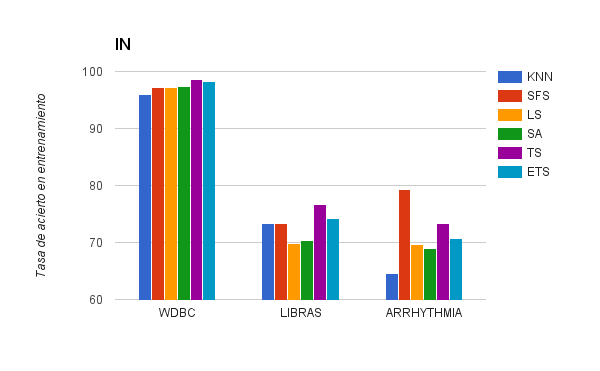
\includegraphics[width=0.5\textwidth]{Resultados/IN-alg}
\caption{Tasa de acierto en el conjunto de entrenamiento}
\end{figure}

De la comparación de la tasa de acierto dentro de la muestra para cada algoritmo y base de datos se desprende que para el problema de clasificación, realizar una selección de características siempre es recomendable, pues se obtiene mayor tasa de acierto que usando sólo KNN. Esto no es así para \texttt{Libras} y búsqueda local y enfriamiento simulado. Esto  se puede deber al elevado número de características y clases, en relación al número de datos. Se aprecia también que la búsqueda tabú mejora los resultados del enfriamiento simulado, con lo que quizá deberíamos pensar en otra exploración de vecinos. Por último, la alta tasa de acierto para SFS en \texttt{Arrhythmia} nos indica que para un número elevado de características y pocas clases, se puede dar que pocas características sean las que contienen la información, y que por tanto ir cogiendo las mejores sea una buena estrategia. Podríamos tener más certeza sobre esto si, por ejemplo, realizamos una búsqueda sobre el espacio de soluciones que sólo tengan un número fijo y pequeño de características (usaríamos otra representación del problema) y comparar los resultados (teniendo en cuenta que esto también sería heurística y que nos costaría tanto o más obtener la mejor selección).

\begin{figure}[h!]
\centering
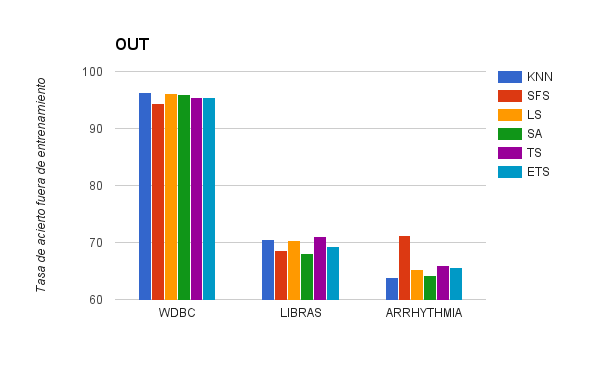
\includegraphics[width=0.5\textwidth]{Resultados/OUT-alg}
\caption{Tasa de acierto fuera del conjunto de entrenamiento}
\end{figure}

Para la tasa de acierto fuera de la muestra, vemos como el orden de los algoritmos es distinto y que ahora no tomar ninguna característica no es una opción a descartar. Esto se explica sencillamente porque los algoritmos de búsqueda han ajustado las características a los datos, y sin embargo, de manera general puede no resultar la mejor opción. Se aprecia ahora que en la base de datos \texttt{WDBC} las tasas son siempre más parejas y mejores (aunque en este caso se requiera una mayor certeza que en el de \texttt{Libras}, por ejemplo) que en las otras. También podemos deducir que para el caso de \texttt{Libras} y \texttt{Arrhythmia} el resultado es más desigual en especial para la búsqueda tabú.

\begin{figure}[h!]
\centering
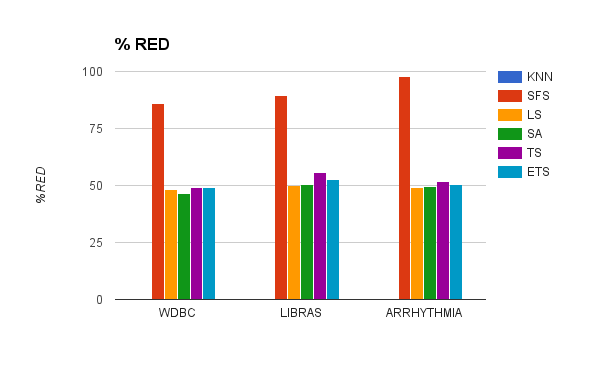
\includegraphics[width=0.5\textwidth]{Resultados/red-alg}
\caption{Porcentaje de reducción de las características}
\end{figure}

En cuanto al porcentaje de reducción, no tiene mucho sentido hacer un análisis más allá de ver cómo el SFS en \texttt{Arrhythmia} tiene un porcentaje muy elevado y es el mejor algoritmo. Esto va en la línea de lo anteriormente comentado. Como la función de evaluación no incluía nada sobre tener el menor número posible de características, los resultados en los demás algoritmos son poco más que aleatorios. Sin embargo, podemos relacionar el buen comportamiento en \texttt{Arrhythmia} de la búsqueda tabú y la ligera mayor reducción del número de características con que ese algoritmo va en la buena dirección.

\begin{figure}[h!]
\centering
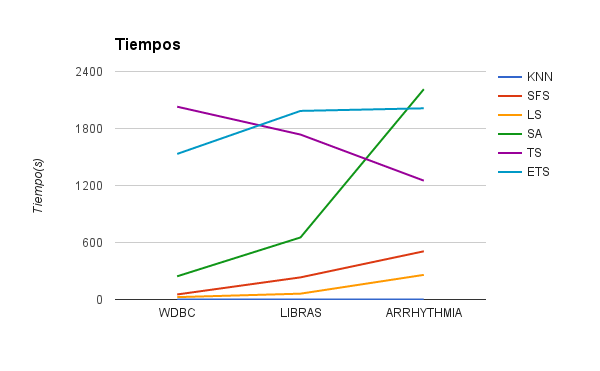
\includegraphics[width=0.5\textwidth]{Resultados/Tiempo}
\caption{Tiempos empleados por el algoritmo}
\end{figure}

En cambio, para los tiempos, incluso teniendo en cuenta que la búsqueda tabú y la tabú extendida no han realizado todas las comprobaciones, sino sólo 5000, el tiempo es mucho mayor que para los demás métodos. Lo que sí es más estable con respecto al tamaño del problema. Mientras que la búsqueda local y el \textit{greedy} SFS tienen un crecimiento más limitado, el enfriamiento simulado aumenta mucho más. La búsqueda tabú tarda un mayor tiempo en \texttt{WDBC}, y esto se puede deber a que la lista tabú coincide en tamaño con el número de características, limitando más la variación de las soluciones, también limitado porque en esta base de datos se encuentra un muy buen resultado en poco tiempo (los datos son más semejantes y hay menos clases) y las mejoras son más difíciles de encontrar.

\section{Bibliografía}
\begin{itemize}
\item \href{http://scikit-learn.org/stable/modules/neighbors.html}{Módulo en \texttt{scikit} para KNN}
\item Para realizar las tablas en \LaTeX: \href{https://www.complang.tuwien.ac.at/doc/texlive-pictures-doc/latex/pgfplots/pgfplotstable.pdf}{Manual PGFPLOTSTABLE}
\end{itemize}
\end{document}
